\subsection{Кардинальный синус}

Рассмотрим семейство функций
\begin{equation}
    f(t) = a \sinc(bt)
    \label{eq:sinc_function}
\end{equation}

\subsubsection{Графики исходных функций}
Графики данной функции при различных значениях $a$ и $b$ представлены на рисунках \ref{fig:sinc_1}, \ref{fig:sinc_2} и \ref{fig:sinc_3}.

\begin{figure}[ht!]
    \centering
    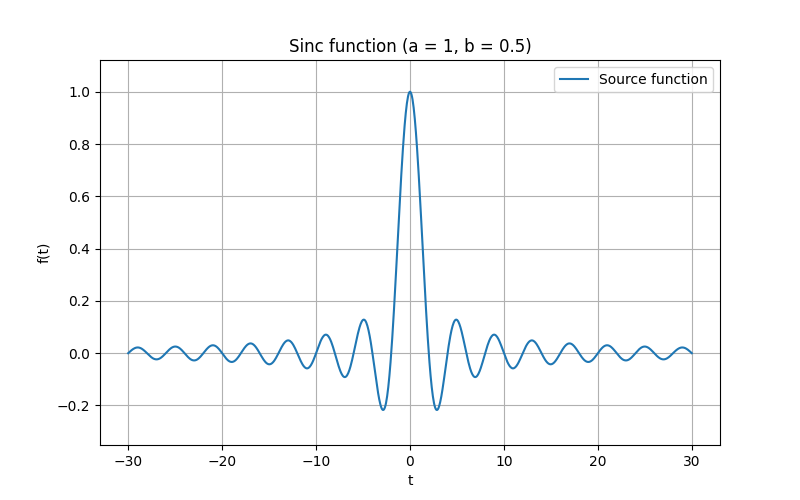
\includegraphics[width=\textwidth]{media/sinc_1.png}
    \caption{График функции $f(t)$ при $a = 1$, $b = 0.5$}
    \label{fig:sinc_1}
\end{figure}

\begin{figure}[ht!]
    \centering
    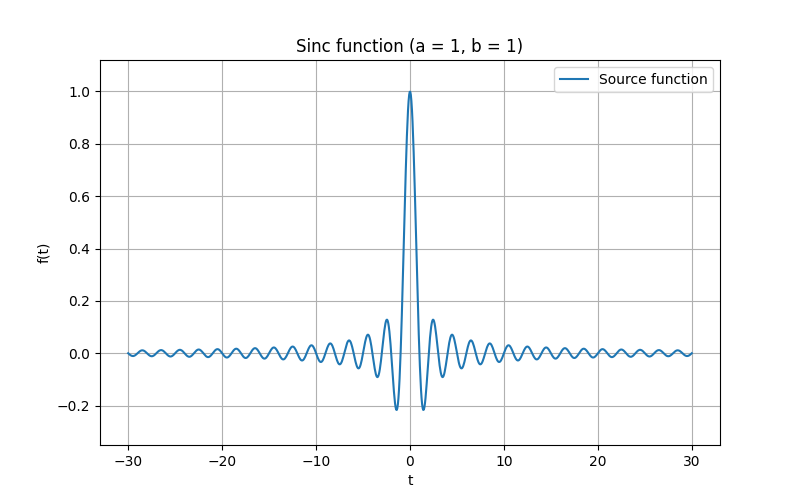
\includegraphics[width=\textwidth]{media/sinc_2.png}
    \caption{График функции $f(t)$ при $a = 1$, $b = 1$}
    \label{fig:sinc_2}
\end{figure}

\begin{figure}[ht!]
    \centering
    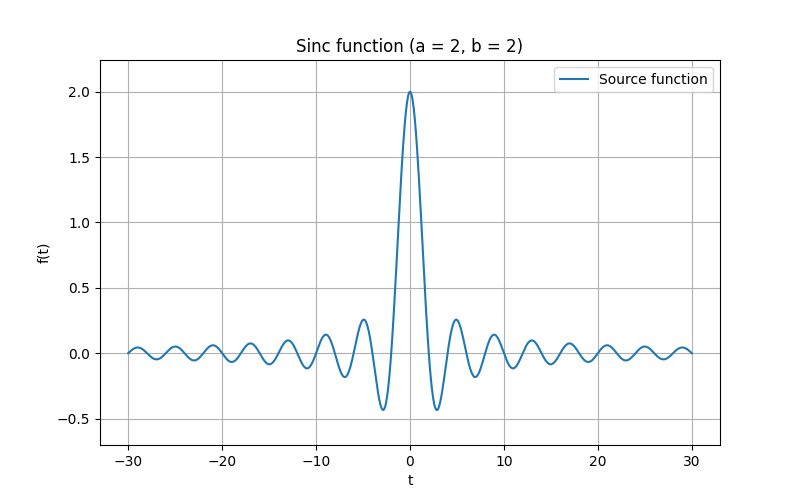
\includegraphics[width=\textwidth]{media/sinc_3.png}
    \caption{График функции $f(t)$ при $a = 2$, $b = 2$}
    \label{fig:sinc_3}
\end{figure}

\FloatBarrier
\subsubsection{Нахождение образа функции}
Согласно формуле \eqref{eq:image_from_function}, Фурье образ функции $f(t)$ задается следующим выражением:

\begin{multline}
    \hat{f}(\omega) = \frac{1}{\sqrt{2\pi}} \int_{-\infty}^{\infty} f(t) e^{-i\omega t} dt = \frac{1}{\sqrt{2\pi}} \int_{-\infty}^{\infty} a \sinc(bt) e^{-i\omega t} dt = \frac{a}{\sqrt{2\pi}} \int_{-\infty}^{\infty} \sinc(bt) e^{-i\omega t} dt = \\
    \frac{\pi a}{\sqrt{2\pi} |b|}\cdot \begin{cases} 0, & \frac{b^2}{\omega^2} \le 1 \\ 1, & \text{otherwise} \end{cases}
\end{multline}

\subsubsection{Графики образов функций}
Графики образов функции \eqref{eq:sinc_function} при различных значениях $a$ и $b$ представлены на рисунках \ref{fig:sinc_1_image}, \ref{fig:sinc_2_image} и \ref{fig:sinc_3_image}.

\begin{figure}[ht!]
    \centering
    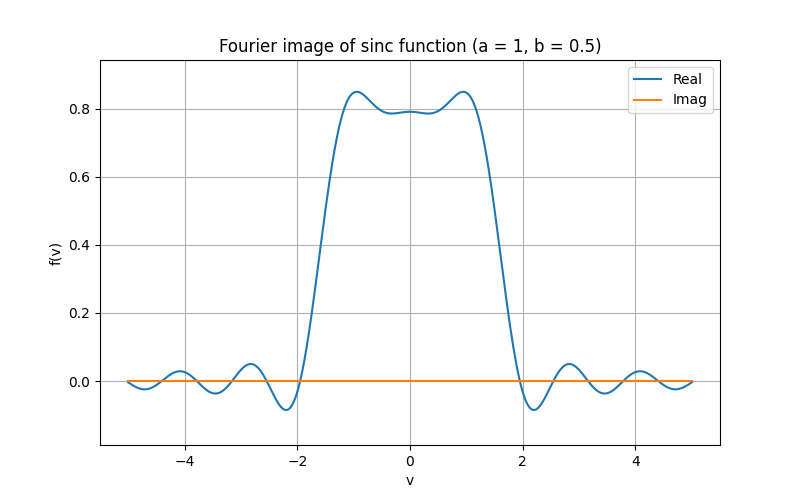
\includegraphics[width=\textwidth]{media/sinc_1_image.png}
    \caption{График образа функции $f(t)$ при $a = 1$, $b = 0.5$}
    \label{fig:sinc_1_image}
\end{figure}

\begin{figure}[ht!]
    \centering
    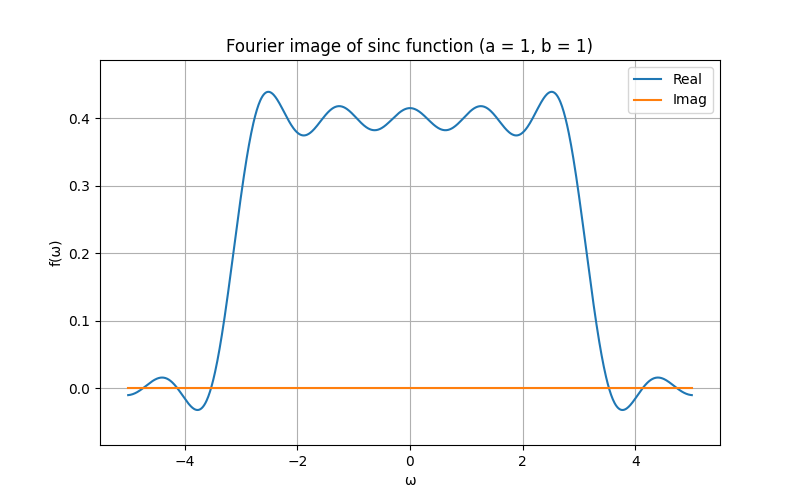
\includegraphics[width=\textwidth]{media/sinc_2_image.png}
    \caption{График образа функции $f(t)$ при $a = 1$, $b = 1$}
    \label{fig:sinc_2_image}
\end{figure}

\begin{figure}[ht!]
    \centering
    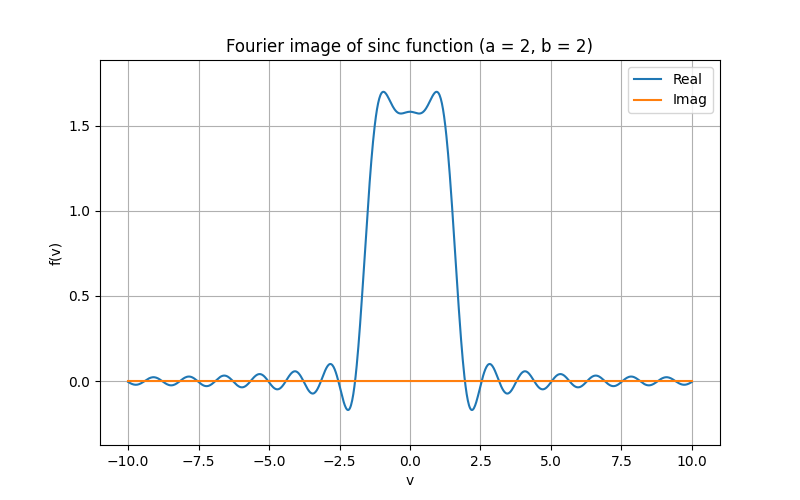
\includegraphics[width=\textwidth]{media/sinc_3_image.png}
    \caption{График образа функции $f(t)$ при $a = 2$, $b = 2$}
    \label{fig:sinc_3_image}
\end{figure}

\FloatBarrier
\subsubsection{Проверка равенства Парсеваля}
Проверим равенство Парсеваля (см. формулу~\eqref{eq:parseval_indentity}). Для этого воспользуемся функцией \texttt{parseval\_check}. 
\begin{table}[ht!]
    \centering
    \begin{tabular}{|c|c|}
        \hline
        $\displaystyle\int_{-100}^{100}{|f(t)|^2}$ & $\displaystyle\int_{-100}^{100}{|\hat{f_1}(\omega)|^2}$ \\
        \hline
        1.9959 & 1.9957 \\
        \hline
    \end{tabular}
    \caption{Результаты проверки равенства Парсеваля для кардинального синуса $f(t)$ при $a = 1$, $b = 0.5$}
    \label{tab:sinc_1_parseval_check}
\end{table}

\begin{table}[ht!]
    \centering
    \begin{tabular}{|c|c|}
        \hline
        $\displaystyle\int_{-100}^{100}{|f(t)|^2}$ & $\displaystyle\int_{-100}^{100}{|\hat{f_2}(\omega)|^2}$ \\
        \hline
        0.9989 & 0.9982 \\
        \hline
    \end{tabular}
    \caption{Результаты проверки равенства Парсеваля для кардинального синуса $f(t)$ при $a = 1$, $b = 1$}
    \label{tab:sinc_2_parseval_check}
\end{table}

\begin{table}[ht!]
    \centering
    \begin{tabular}{|c|c|}
        \hline
        $\displaystyle\int_{-100}^{100}{|f(t)|^2}$ & $\displaystyle\int_{-100}^{100}{|\hat{f_3}(\omega)|^2}$ \\
        \hline
        1.9989 & 1.9996 \\
        \hline
    \end{tabular}
    \caption{Результаты проверки равенства Парсеваля для кардинального синуса $f(t)$ при $a = 2$, $b = 2$}
    \label{tab:sinc_3_parseval_check}
\end{table}

Видим, что во всех случаях равенство Парсеваля выполняется с хорошей точностью. 

\subsubsection{Анализ результатов}
Коэффициент $a$ влияет на амплитуду функции, а коэффициент $b$ влияет на частоту колебаний. При увеличении $a$ амплитуда увеличивается, при увеличении $b$ частота увеличивается.
Видим, что график образа функции похож на график квадратичной функции, это связано с тем, что образ квадратичной функции как раз является кардинальным синусом, а значит, что образ кардинального синуса является квадратичной функцией.

Принцип неопределенности проявляется здесь ровно так же, как и в случае с квадратичной функцией. При уменьшении ширины кардинального синуса увеличивается ширина его образа. 